\documentclass[11pt,a4paper]{article}
\usepackage[T1]{fontenc}
\usepackage[margin=2.3cm]{geometry}
\usepackage{amsmath,amssymb}
\usepackage{graphicx}
\usepackage[dvipsnames]{xcolor}
\usepackage{enumitem}
\usepackage[colorlinks=true,linkcolor=blue,urlcolor=blue]{hyperref}
\setlength{\parskip}{0.6em}
\setlength{\parindent}{0pt}
\begin{document}

\begin{center}{\LARGE\bfseries openfatigue}\\[0.4em]{\large Predict how many load cycles a part survives, from the paper clip to the S-N curve.}\\[0.2em]\small PAN IIT OSS explainer \textbullet{} diploma / undergraduate to advanced undergraduate (levels 5-6)\end{center}

\section*{Why this exists}
Most broken machine parts did not fail because of one big load. They failed because a modest load was repeated millions of times. This explainer shows the mathematics behind that, using logarithms, a few power laws and some counting, so you can build the estimate yourself.

\section*{The end goal}
Predict how many load cycles a part survives (S-N curve). The end goal is predicting how many load cycles a part survives, with the S-N curve at the centre: from a stress amplitude to a life, with mean stress, notches, variable loads, crack growth and scatter. All models here are simplified and illustrative; real design of structures, vehicles and aircraft follows tested data, standards and qualified engineers.

\section*{How the three sessions build up}
\begin{enumerate}[nosep]
\item \textbf{Session 1: Repeated loads break what one load cannot} (Level 1, conceptual interactive model, 60 min).
\item \textbf{Session 2: The S-N curve as an equation: mean stress and notches} (Level 2, mathematical engineering model, 75 min).
\item \textbf{Session 3: Variable loads, cracks and scatter: a life estimate} (Level 3, simulation and validation, 90 min).
\end{enumerate}

\section{Session 1: Repeated loads break what one load cannot}

\subsection*{A. Real-world problem}
Bend a paper clip once and it springs back. Bend it back and forth and it snaps, even though no single bend was harder than the first. Bridges, axles, springs and aircraft skins fail in the same quiet way: the damage builds up cycle after cycle. Engineers must answer a practical question: if a part sees a given stress again and again, how many cycles does it survive? (Educational model with illustrative numbers; never use it to design a real part.)

\subsection*{B. Concept and theory}
A rotating shaft that is bent sees each surface point go from pull to push and back: the stress is a wave, stress = S\_m + S\_a sin(2 pi f t), with mean S\_m, amplitude S\_a and frequency f. One full wave is one cycle. The range is twice the amplitude. If many identical bars are each tested at a different amplitude and the cycles N until they break are counted, the points fall close to a straight line when both axes are drawn on logarithmic scales. That line is Basquin's relation S\_a = A N\textasciicircum{}b. The exponent b is negative (more stress, fewer cycles) and for typical steels it is about -0.1; our illustrative steel has b = -0.085, because the line is drawn through 0.9 S\_u at 1000 cycles and through the endurance limit S\_e at one million cycles. Many steels show an endurance limit, about half of S\_u, below which the test bars survive a very long time.

\begin{itemize}[nosep]
\item S\_a: stress amplitude (half the range) (MPa)
\item S\_u: ultimate (one-pull) strength, 600 here (MPa)
\item S\_e: endurance limit, 300 here (0.5 S\_u) (MPa)
\item N: cycles to failure (cycles)
\item A, b: constants of the S-N line; A = 972 MPa, b = -0.085 here (MPa, no unit)
\item f: loading frequency (Hz (cycles per second))
\end{itemize}

\begin{equation*}
S(t)=S_m+S_a\sin(2\pi f t),\qquad \Delta S = 2S_a
\end{equation*}

\begin{equation*}
S_a=A\,N^{\,b},\qquad N=\left(\frac{S_a}{A}\right)^{1/b}
\end{equation*}

\begin{equation*}
b=-\frac{1}{3}\log_{10}\frac{0.9\,S_u}{S_e},\qquad A=\frac{(0.9\,S_u)^2}{S_e}
\end{equation*}

\begin{equation*}
t_{\mathrm{fail}}=\frac{N}{f}
\end{equation*}

\begin{center}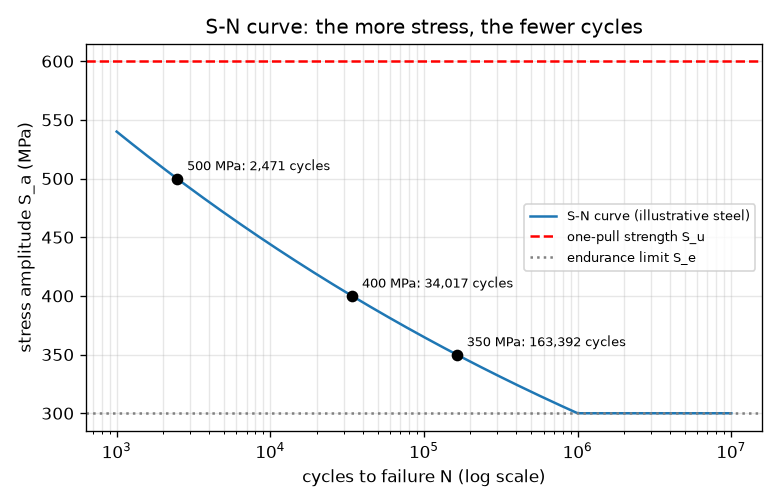
\includegraphics[width=0.85\linewidth]{figures/s01_sn_curve.png}\\\small The S-N curve of the illustrative steel with three marked operating points and the endurance limit.\end{center}

\subsection*{E. Worked example}
A steel bar (S\_u = 600 MPa, S\_e = 300 MPa, so A = 972 MPa and b = -0.085) is loaded with a fully reversed amplitude of 400 MPa at 10 Hz. How many cycles does it survive and for how long does it run?
\begin{enumerate}[nosep]
\item Check the model applies: 400 MPa is above S\_e = 300 MPa, so the life is finite, and below S\_u = 600 MPa, so one pull would not break it.
\item N = (S\_a / A)\textasciicircum{}(1/b) = (400 / 972)\textasciicircum{}(1 / -0.0851). Here 400 / 972 = 0.4115, log10(0.4115) = -0.3856, and 1/b = -11.75.
\item log10 N = -0.3856 x -11.75 = 4.53, so N = 10\textasciicircum{}4.53 = 34,000 cycles (34,017 with more digits).
\item Running time = N / f = 34,017 / 10 = 3,402 s = 56.7 minutes.
\item Sanity check: 400 MPa lies between the 540 MPa at 1000 cycles and the 300 MPa at one million cycles, so a life between 1,000 and 1,000,000 cycles is right.
\end{enumerate}
\textbf{Answer.} About 34,000 cycles, which is about 57 minutes at 10 Hz.

\subsection*{F. Questions}
\begin{enumerate}[nosep]
\item \textbf{Conceptual.} Why can a part break under a repeated stress that is smaller than the stress needed to break it in one pull? What does the part 'remember' from one cycle to the next?
\item \textbf{Numerical.} The same steel is loaded at an amplitude of 350 MPa and 20 Hz. Find the number of cycles to failure and the running time in hours. Check that the answer is sensible.
\item \textbf{Graph and simulation interpretation.} On the S-N graph, the amplitude is raised from 400 MPa to 500 MPa, a rise of 25 percent. By what factor does the life fall? What does the steep curve tell a designer?
\item \textbf{Design and optimisation challenge.} A rotating bar sees an amplitude of 450 MPa. It must run 8 hours a day at 10 Hz for 30 days. (a) How many cycles is that? (b) How long does it last at 450 MPa? (c) In bending, stress goes as 1/d\textasciicircum{}3 (d = diameter). By what factor must the diameter grow to bring the stress down to the endurance limit?
\end{enumerate}

\section{Session 2: The S-N curve as an equation: mean stress and notches}

\subsection*{A. Real-world problem}
A shaft carries a pulley load and turns at 1500 revolutions per minute (25 per second): each surface point is pulled and pushed once per revolution, so about 11 hours of running make a million cycles. What diameter keeps it safe for 10\textasciicircum{}6 cycles and beyond, with a margin? On the way we meet the two things that shorten life most: a mean stress (a load that never fully reverses) and a notch such as a hole or sharp shoulder. All numbers are illustrative; this is a simplified model, not a design method for real shafts.

\subsection*{B. Concept and theory}
Basquin's relation S\_a = A N\textasciicircum{}b is a straight line on log-log axes. We anchor it at 0.9 S\_u for 1000 cycles and at S\_e for 10\textasciicircum{}6 cycles, which gives b = -(1/3) log10(0.9 S\_u / S\_e) and A = (0.9 S\_u)\textasciicircum{}2 / S\_e. For the polished bar (S\_e = 300 MPa) b = -0.085; for a real part with a lower endurance limit (210 MPa, which is 0.7 of 300 for surface finish and size, an illustrative factor) the line is steeper, b = -0.137. Both are close to the 'typical' value of about -0.1 quoted for steels. Mean stress: a tensile mean opens cracks and shortens life; the Goodman line S\_a / S\_e + S\_m / S\_u = 1 separates combinations below it (indefinite life predicted) from those above it. For a load with mean we convert to the equivalent fully reversed amplitude S\_eq = S\_a / (1 - S\_m / S\_u) and use the S-N line. Notches: near a hole or corner the local stress is K\_t times the nominal one. For a hole in a wide plate under uniaxial stress the exact elastic hoop stress at the edge is S (1 - 2 cos 2 theta), which peaks at 3 S at theta = 90 degrees from the load direction, so K\_t = 3. We apply K\_t to both amplitude and mean (a simple conservative choice). Caveat: the endurance limit is a feature of many steels; aluminium and many other metals have no true endurance limit, and their S-N curve keeps falling, so a fatigue strength at a stated life (for example 10\textasciicircum{}8 cycles) is used instead.

\begin{itemize}[nosep]
\item S\_a, S\_m: stress amplitude and mean stress (MPa)
\item S\_u, S\_e: ultimate strength (600) and endurance limit (300 for a bar, 210 for the part) (MPa)
\item S\_eq: equivalent fully reversed amplitude (MPa)
\item K\_t: theoretical stress concentration factor (no unit)
\item M: bending moment on the shaft (N m)
\item d: shaft diameter (m (mm in tables))
\item n: safety factor on stress (no unit)
\item A, b: constants of the S-N line (MPa, no unit)
\end{itemize}

\begin{equation*}
S_a=A\,N^{b},\quad b=-\tfrac13\log_{10}\frac{0.9S_u}{S_e},\quad A=\frac{(0.9S_u)^2}{S_e}
\end{equation*}

\begin{equation*}
\frac{S_a}{S_e}+\frac{S_m}{S_u}=1,\qquad S_{eq}=\frac{S_a}{1-S_m/S_u}
\end{equation*}

\begin{equation*}
\sigma_\theta(r=a)=\sigma\,(1-2\cos 2\theta)\;\Rightarrow\; K_t=\frac{\sigma_{\max}}{\sigma_{nom}}=3
\end{equation*}

\begin{equation*}
S_a=\frac{32M}{\pi d^3},\qquad d=\left(\frac{32\,M\,n\,K_t}{\pi\,S_{e,part}}\right)^{1/3}
\end{equation*}

\begin{center}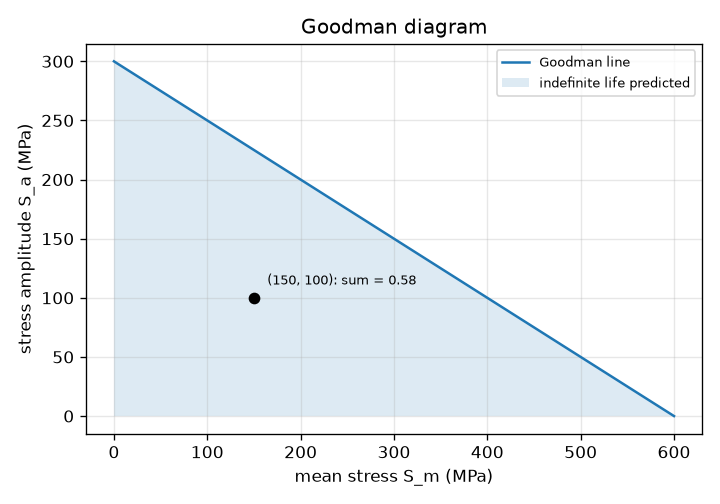
\includegraphics[width=0.85\linewidth]{figures/s02_goodman.png}\\\small The Goodman line and the indefinite-life region, with one operating point.\end{center}

\subsection*{E. Worked example}
A shaft carries a steady bending moment M = 200 N m. Choose its diameter for 10\textasciicircum{}6 cycles and beyond with a safety factor n = 2 on stress, for a plain shaft (K\_t = 1) and for a shaft with a shoulder (K\_t = 2). The part endurance limit is 210 MPa.
\begin{enumerate}[nosep]
\item Require K\_t S\_a \textless{}= S\_e,part / n = 210 / 2 = 105 MPa for K\_t = 1.
\item d = (32 M n K\_t / (pi S\_e,part))\textasciicircum{}(1/3) = (32 x 200 x 2 x 1 / (pi x 210e6))\textasciicircum{}(1/3) = (1.940e-5)\textasciicircum{}(1/3) m = 0.02687 m = 26.87 mm. Round up to 27 mm.
\item Check the 27 mm shaft: S\_a = 32 x 200 / (pi x 0.027\textasciicircum{}3) = 103.5 MPa, so the margin is 210 / 103.5 = 2.03, as required.
\item With a shoulder, K\_t = 2: d = 26.87 x 2\textasciicircum{}(1/3) = 33.86 mm. A sharper corner costs 7 mm of diameter.
\item Sanity check: a thinner 20 mm shaft has S\_a = 254.6 MPa (above 210), so on the part's S-N line it fails after about 244,000 cycles, less than 10\textasciicircum{}6. The 27 mm shaft has an indefinite life in this model.
\end{enumerate}
\textbf{Answer.} d = 26.87 mm, so use 27 mm (stress 103.5 MPa, margin 2.03); with a shoulder with K\_t = 2 use 33.86 mm, about 34 mm.

\subsection*{F. Questions}
\begin{enumerate}[nosep]
\item \textbf{Conceptual.} Why does a tensile mean stress shorten fatigue life, and why is the same load safe for steel but not necessarily for aluminium when it lies below the endurance limit?
\item \textbf{Numerical.} A load has S\_a = 240 MPa and S\_m = 250 MPa on the illustrative steel (S\_u = 600, S\_e = 300). Find the Goodman equivalent amplitude and the life. What would the life be with zero mean?
\item \textbf{Graph and simulation interpretation.} On the Goodman diagram the point (S\_m, S\_a) = (300, 150) MPa is plotted. Where is it, and what does the Goodman sum say? What happens if the amplitude rises slightly?
\item \textbf{Design and optimisation challenge.} Design: a shaft carries M = 150 N m, has a shoulder fillet with K\_t = 1.5, and must have a safety factor of 2 on stress for indefinite life (part endurance limit 210 MPa). Choose a diameter, compare 25 mm and 28 mm, and say what happens at 22 mm. State the trade-off.
\end{enumerate}

\section{Session 3: Variable loads, cracks and scatter: a life estimate}

\subsection*{A. Real-world problem}
A bracket on a vibrating machine does not see a neat sine wave: it sees vibration, start-ups and now and then a hard knock. How many shifts will it last, and how often must it be inspected for cracks? Real life prediction stacks several ideas: count the cycles, add up their damage, and, once a crack exists, grow it. And two parts made alike never fail together. (Educational model with illustrative numbers; never a method for certifying real or safety-critical parts.)

\subsection*{B. Concept and theory}
Rainflow counting turns a history into cycles. After reducing it to its turning points (reversals), the standard three-point rule (ASTM E1049) keeps a stack: if the newest range X is at least the previous range Y, then Y is a closed loop and counts as one full cycle, or one half cycle if it contains the start of the history; the leftover points at the end count as half cycles. Miner's rule is the standard linear damage rule: a block of n\_i cycles at a level with life N\_i uses up n\_i / N\_i of the life, and failure is predicted when D = sum n\_i / N\_i reaches 1. It ignores load order and interaction between levels, and in tests D at failure scatters widely, roughly 0.3 to 3, so it is an estimate. Crack growth follows Paris' law da/dN = C (delta K)\textasciicircum{}m with delta K = Y delta\_sigma sqrt(pi a); for constant Y and m not equal to 2 the cycles from a0 to the critical length a\_c are N = (a\_c\textasciicircum{}(1 - m/2) - a0\textasciicircum{}(1 - m/2)) / (C Y\textasciicircum{}m delta\_sigma\textasciicircum{}m pi\textasciicircum{}(m/2) (1 - m/2)). The critical length comes from K\_max = K\_Ic. Fatigue life is lognormal: log10 N is normal around its prediction. Because N goes as stress to the power 1/b, a stress change by a factor r changes life by r\textasciicircum{}(1/b): note the exponent is 1/b, not b.

\begin{itemize}[nosep]
\item range, mean: range and mean of a rainflow cycle (MPa)
\item n\_i, N\_i: applied cycles and life at level i (cycles)
\item D: Miner damage sum (no unit)
\item a, a0, a\_c: crack length, initial and critical (m)
\item delta K: stress-intensity range (MPa sqrt(m))
\item C, m: Paris constants (6.9e-12 and 3 for steel in these units) (see text)
\item Y: crack shape factor (1.12, small edge crack) (no unit)
\item K\_Ic: fracture toughness (50 here) (MPa sqrt(m))
\item sigma\_log10: scatter of log10 N (0.3 here) (no unit)
\end{itemize}

\begin{equation*}
D=\sum_i \frac{n_i}{N_i},\qquad \text{failure predicted at } D=1
\end{equation*}

\begin{equation*}
\frac{da}{dN}=C(\Delta K)^m,\qquad \Delta K=Y\,\Delta\sigma\sqrt{\pi a}
\end{equation*}

\begin{equation*}
N=\frac{a_c^{\,1-m/2}-a_0^{\,1-m/2}}{C\,Y^m\,\Delta\sigma^m\,\pi^{m/2}\,(1-m/2)},\quad m\neq 2
\end{equation*}

\begin{equation*}
a_c=\left(\frac{K_{Ic}}{Y\,\sigma_{\max}\sqrt{\pi}}\right)^2,\qquad \frac{N_2}{N_1}=r^{1/b}
\end{equation*}

\begin{center}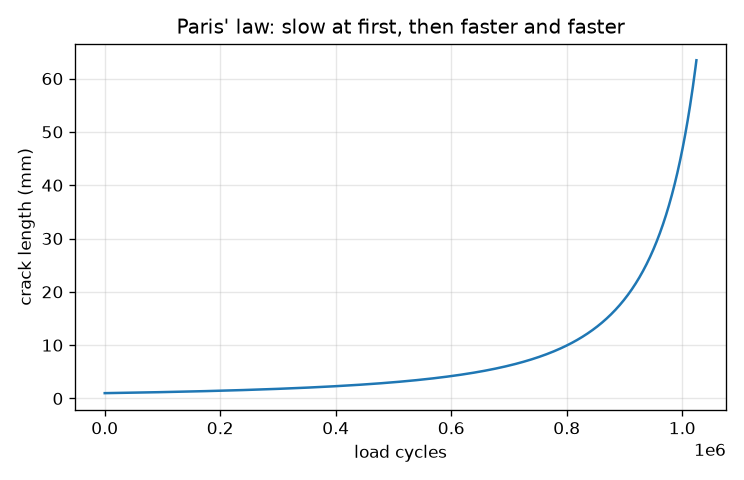
\includegraphics[width=0.85\linewidth]{figures/s03_crack_growth.png}\\\small Paris' law crack growth from 1 mm to the critical length: slow at first, then accelerating.\end{center}

\subsection*{E. Worked example}
A part has seen 10,000 cycles at an amplitude of 400 MPa and 50,000 cycles at 350 MPa (fully reversed, S\_u = 600 MPa, S\_e = 300 MPa). By Miner's rule, how much of its life is used, and how many more cycles at 400 MPa can it take?
\begin{enumerate}[nosep]
\item Lives from the S-N line: N(400) = 34,017 cycles and N(350) = 163,392 cycles.
\item Damage at 400 MPa: 10,000 / 34,017 = 0.294. Damage at 350 MPa: 50,000 / 163,392 = 0.306.
\item Total D = 0.294 + 0.306 = 0.600, so 60 percent of the life is used and 0.400 remains.
\item More cycles at 400 MPa: 0.400 x 34,017 = 13,607 cycles (about 13,600).
\item Sanity check: if the order were reversed the sum would be the same, which is exactly Miner's weakness: real parts care about order.
\end{enumerate}
\textbf{Answer.} D = 0.600 used; about 13,600 more cycles at 400 MPa remain.

\subsection*{F. Questions}
\begin{enumerate}[nosep]
\item \textbf{Conceptual.} Give two reasons why Miner's rule can be wrong, and say whether ignoring cycles below the endurance limit is safe when large overloads are also present.
\item \textbf{Numerical.} An edge crack (Y = 1.12) in a part sees a stress range of 80 MPa (zero to maximum). Using C = 6.9e-12, m = 3 and K\_Ic = 50 MPa sqrt(m), find delta K for a0 = 2 mm, the critical length and the life in cycles.
\item \textbf{Graph and simulation interpretation.} In the scatter histogram the 5th percentile life is 31,000 cycles and the 95th is 311,000 for a median of 100,000. What does the spread say about testing one part, and what ratio of 95th to 5th percentile do you read off?
\item \textbf{Design and optimisation challenge.} Design: the bracket's life is 4,998 shifts with 6 hard knocks per shift. A customer needs at least 4,000 shifts. How many knocks per shift may the machine produce at most? And the inspection method can find a crack of 1 mm instead of 0.5 mm: what happens to the interval, and what if it can only find 2 mm?
\end{enumerate}

\section{Real-world mini-project}
\textbf{Bracket life and inspection interval from a load history.} A bracket on a vibrating machine has a measured hot-spot stress history for one shift (here a synthetic one from \texttt{bracket\_history()}: steady vibration, 10 start-ups and a few hard knocks). Count its cycles with \texttt{rainflow}, add the damage with \texttt{miner\_damage}, and turn it into a life in shifts. Then use Paris' law to find the number of shifts a crack needs to grow from a detectable size of 0.5 mm to the critical size, divide by a safety factor of 3, and report an inspection interval. Finally a customer requires a life of at least 4,000 shifts: find the largest number of hard knocks per shift (0 to 14) the machine may produce.

\section{The path ahead}
\begin{enumerate}[nosep]
\item \textbf{Session 4: Fatigue notch factor K\_f.} A function that returns K\_f between 1 and K\_t from the notch radius and the material, used in the plate-with-hole life.
\item \textbf{Session 5: Beyond the straight line: low cycles and the knee.} A strain-life curve with an elastic and a plastic part, joined to the S-N line.
\item \textbf{Session 6: Reliability design life.} A function that gives the design life for a chosen reliability from the median life and the log scatter.
\item \textbf{Session 7: Overload retardation in crack growth.} A crack growth integrator that tracks the overload plastic zone and slows growth behind it.
\item \textbf{Session 8: Reproduce the Target: initiation plus propagation.} An animation with an S-N operating point, a plate with a growing crack and two bars.
\end{enumerate}

\section{Answers and hints}

\subsection*{Session 1}
\begin{enumerate}[nosep]
\item \textbf{Conceptual.} Hint: Think of the paper clip: what changes inside it with every bend? Solution: Each cycle causes a tiny amount of permanent damage, mostly at microscopic places where stress is highest (a scratch, a corner, a grain boundary). The damage is not undone when the load is removed, so it accumulates until a crack forms and grows. One pull below S\_u causes no such accumulating damage, but many repetitions do. The part 'remembers' its accumulated damage, not the load itself.
\item \textbf{Numerical.} Hint: N = (S\_a / A)\textasciicircum{}(1/b) with A = 972 MPa and b = -0.0851; time = N / f. Solution: N = (350 / 972)\textasciicircum{}(-11.75) = 163,392 cycles (about 163,000). Time = 163,392 / 20 = 8,170 s = 2.27 hours. Sanity check: 350 MPa lies between 300 MPa (one million cycles) and 400 MPa (34,000 cycles), so the life must lie between those two values: it does.
\item \textbf{Graph and simulation interpretation.} Hint: Read N at both stresses (or compute them) and divide. Solution: N falls from 34,017 to 2,471 cycles, a factor of 13.8 (about 14 times shorter). A 25 percent rise in stress costs more than an order of magnitude of life: fatigue life is very sensitive to stress, so small stress reductions (a larger radius, a slightly thicker section) buy a lot of life.
\item \textbf{Design and optimisation challenge.} Hint: (a) cycles = hours x 3600 x frequency. (b) use the S-N relation. (c) 450 / 300 = (d\_new / d\_old)\textasciicircum{}3. Solution: (a) 8 x 3600 x 10 x 30 = 8,640,000 cycles. (b) N at 450 MPa = 8,522 cycles, only 14.2 minutes at 10 Hz. So the bar fails on day one. (c) The stress must fall by 450 / 300 = 1.5, so d\_new / d\_old = 1.5\textasciicircum{}(1/3) = 1.145: a diameter 14.5 percent larger brings the amplitude to 300 MPa, the endurance limit. Assumptions: perfect bar, no notches, no safety margin. A real design would add a margin (Session 2).
\end{enumerate}

\subsection*{Session 2}
\begin{enumerate}[nosep]
\item \textbf{Conceptual.} Hint: Think about what a tensile mean does to a crack, and about what the S-N curve of aluminium does at high cycles. Solution: A tensile mean stress holds cracks open and raises the peak stress of every cycle, so each cycle does more damage; the Goodman line captures this by lowering the allowed amplitude as the mean rises. Steels often show an endurance limit, a flat S-N curve below which life is practically unlimited; aluminium has no true endurance limit, its curve keeps falling, so a load below any chosen 'limit' still fails eventually after enough cycles (design for a stated life such as 10\textasciicircum{}8 cycles).
\item \textbf{Numerical.} Hint: S\_eq = S\_a / (1 - S\_m / S\_u); then N = (S\_eq / 972)\textasciicircum{}(1/b). Solution: S\_eq = 240 / (1 - 250/600) = 240 / 0.5833 = 411.4 MPa. N = (411.4 / 972)\textasciicircum{}(-11.75) = 24,430 cycles (about 24,400). With zero mean, 240 MPa is below S\_e = 300 MPa, so the life is indefinite. The tensile mean turned a safe load into a failure after about 24,000 cycles.
\item \textbf{Graph and simulation interpretation.} Hint: Compute 150 / 300 + 300 / 600. Solution: 150 / 300 + 300 / 600 = 0.5 + 0.5 = 1.0, so the point lies exactly on the Goodman line: no margin at all. A slightly larger amplitude puts it above the line, into the zone where finite life is predicted. Practical meaning: points near the line should be treated as unsafe once the scatter of real data is included.
\item \textbf{Design and optimisation challenge.} Hint: d = (32 M n K\_t / (pi S\_e,part))\textasciicircum{}(1/3), then check the margin 210 / (K\_t S\_a) at the diameters you consider. Solution: d = (32 x 150 x 2 x 1.5 / (pi x 210e6))\textasciicircum{}(1/3) = 27.95 mm, so choose 28 mm. Margins: 25 mm gives 210 / 146.7 = 1.43 (below the required 2), 28 mm gives 210 / 104.4 = 2.01 (meets it). At 22 mm the local stress is 215.2 MPa, just above 210, so the life is finite: about 835,000 cycles, below 10\textasciicircum{}6. Without the fillet (K\_t = 1) 24.41 mm would do. Trade-off: a gentler fillet radius lowers K\_t and saves diameter, weight and cost, but needs more space and machining. Assumptions: constant bending moment, 0.7 factor, no mean stress.
\end{enumerate}

\subsection*{Session 3}
\begin{enumerate}[nosep]
\item \textbf{Conceptual.} Hint: Think of load order, residual stress and what a large overload does to a crack. Solution: (1) Miner ignores the order of loads: a large cycle early can create residual stress or a small crack that makes later small cycles damaging, so cycles below S\_e that are harmless alone become damaging. (2) It assumes damage is linear and independent of level, but real cracks grow faster as they get longer, and in tests the sum at failure ranges roughly from 0.3 to 3. So ignoring cycles below S\_e is not safe in general when overloads occur: those cycles can then contribute. For our bracket the 'extend' and 'ignore' modes differ little (4,998 against 5,046 shifts) because the overloads dominate, but that has to be checked, not assumed.
\item \textbf{Numerical.} Hint: delta K = Y delta\_sigma sqrt(pi a); a\_c = (K\_Ic / (Y sigma\_max sqrt(pi)))\textasciicircum{}2; then the closed form with m = 3. Solution: delta K at 2 mm = 1.12 x 80 x sqrt(pi x 0.002) = 7.10 MPa sqrt(m). a\_c = (50 / (1.12 x 80 x 1.7725))\textasciicircum{}2 = 0.0991 m = 99.1 mm. Life from the closed form = 1,388,293 cycles, about 1.39 million. Sanity check: delta K at a0 is far below the toughness 50, so most of the life is spent while the crack is still short.
\item \textbf{Graph and simulation interpretation.} Hint: Divide the two percentiles; compare with 10\textasciicircum{}(2 x 1.645 x 0.3). Solution: The ratio is about 9.9, nearly a factor 10 (theory for a normal log10 N with width 0.3: 10\textasciicircum{}(2 x 1.645 x 0.3) = 9.7). One test part could fail at a third of the median or last three times longer, so one test says very little: designers use many parts and a low-percentile life. The 1st percentile life is only about 0.19 of the median.
\item \textbf{Design and optimisation challenge.} Hint: Run \texttt{bracket\_history(n\_knocks=k)} with \texttt{rainflow} and \texttt{miner\_damage} for k = 0 to 14, and \texttt{inspection\_interval\_shifts(stress, a\_detect)} for 0.5, 1 and 2 mm. Solution: Life against knocks: 0 gives 56,607 shifts, 6 give 4,998, 7 give 4,310, 8 give 3,799, 12 give 2,781. So at most 7 knocks per shift keep life at 4,000 shifts or more. The inspection interval (shifts for a crack to grow from the detectable length to the critical length 3.13 mm, divided by 3) is 252 shifts for 0.5 mm, 129 for 1 mm and only 42 for 2 mm: a poor detection method leaves almost no growth window, so inspections must be far more frequent. Trade-offs: fewer knocks (better operation or a damper), better inspection (cost), or a stronger bracket (a lower hot-spot stress). Assumptions: synthetic history, Miner's rule, constant Paris constants, safety factor 3.
\end{enumerate}

\section{How to join}
Read \texttt{CONTRIBUTING.md} in the repository, then pick an issue labelled \texttt{good first issue}. Repository: \url{https://github.com/KrunalPanchal1995/openfatigue}

\end{document}
